\documentclass[UTF-8, a4paper, 10pt]{article}

\usepackage{xeCJK}
\usepackage{graphicx}
\graphicspath{{figure/}}
\usepackage[unicode]{hyperref}
\hypersetup{colorlinks=true,linkcolor=black}
\usepackage{cite}
\usepackage{indentfirst}
\usepackage{amsmath}
\numberwithin{equation}{section}
\usepackage{listings}
\usepackage{xcolor}
\usepackage{fontspec}
\usepackage{courier}
\usepackage{booktabs}
\usepackage{tikz-timing}

\lstset{
    basicstyle=\scriptsize\ttfamily,
    numbers=left,                                        % 在左侧显示行号
    keywordstyle=\color[RGB]{40,40,255},                 % 设定关键字颜色
    frame=trbl,
    numberstyle=\scriptsize\color{darkgray},           % 设定行号格式
    commentstyle=\it\color[RGB]{0,96,96},                % 设置代码注释的格式
    stringstyle=\ttfamily\slshape\color[RGB]{128,0,0},   % 设置字符串格式
    showstringspaces=false,                              % 不显示字符串中的空格
    language=python,                                     % 设置语言
}


\linespread{1.0}
\setlength{\parskip}{0.5\baselineskip}

\makeatletter
\let\@afterindentfalse\@afterindenttrue
\@afterindenttrue
\makeatother
\setlength{\parindent}{2em}

\addtolength{\topmargin}{-70pt}
\setlength{\oddsidemargin}{0.63cm}
\setlength{\evensidemargin}{\oddsidemargin}
\setlength{\textwidth}{15.66cm}
\setlength{\textheight}{25.00cm}

\newcommand{\chuhao}{\fontsize{42pt}{\baselineskip}\selectfont}
\newcommand{\xiaochuhao}{\fontsize{36pt}{\baselineskip}\selectfont}
\newcommand{\yihao}{\fontsize{28pt}{\baselineskip}\selectfont}
\newcommand{\erhao}{\fontsize{21pt}{\baselineskip}\selectfont}
\newcommand{\xiaoerhao}{\fontsize{18pt}{\baselineskip}\selectfont}
\newcommand{\sanhao}{\fontsize{15.75pt}{\baselineskip}\selectfont}
\newcommand{\sihao}{\fontsize{14pt}{\baselineskip}\selectfont}
\newcommand{\xiaosihao}{\fontsize{12pt}{\baselineskip}\selectfont}
\newcommand{\wuhao}{\fontsize{10.5pt}{\baselineskip}\selectfont}
\newcommand{\xiaowuhao}{\fontsize{9pt}{\baselineskip}\selectfont}
\newcommand{\liuhao}{\fontsize{7.875pt}{\baselineskip}\selectfont}
\newcommand{\qihao}{\fontsize{5.25pt}{\baselineskip}\selectfont}

\begin{document}

\begin{titlepage}
    \begin{center}
    \phantom{Start!}
	\vspace{2cm}
	
\includegraphics[width=350pt]{HUST.pdf} \\
    \vspace{1cm}
     \center{
       	  \textbf{\yihao 实\quad 验\quad 报\quad 告}\\
       	  \vspace{0.5cm}
          \textbf{\sanhao (2017 / 2018学年\quad 第2学期)}
      }
      \vspace{2.5cm}
      \begin{table}[!hbp]
      \centering
      \renewcommand\arraystretch{1.5}
     	\begin{tabular}{|c|c|}
     		\hline
     		课程名称 & 机器学习导论 \\
     		\hline
     		实验名称 & ~~~~~~Location Assignment~~~~~~ \\
     		\hline
     		实验时间&\multicolumn{1}{c|}{2018年6月20日}\\
     		\hline
     		指导教师 & 王邦 \\
     		\hline
     		\end{tabular}     		
       \end{table}
       \vspace{2cm}
      \begin{table}[htbp]
      \centering
      \renewcommand\arraystretch{1.5}
     	\begin{tabular}{|c|c|c|c|}
     		\hline
            \qquad ~~姓名~~~~~  & \qquad ~~游浩然~~~~~  & \qquad 学号~~~~~ & \qquad U201515429~~~~~ \\
     		\hline
     		\end{tabular}
       \end{table}
       \date{2018年5月29日}
     \end{center}
\end{titlepage}

\section{问题重述}
\begin{itemize}
  \item 如下图 \ref{nanyi} 所示,为南一楼二楼局部区域室内布局图。绿色区域为数据采集区域。共包括四个教室和室外的走廊。如下所示建立坐标轴,规定左上角坐标为(0,0)。现收集各坐标的不同BSSID的信号强度值,拟据此推断其位置坐标。
      \begin{figure}[!htbp]
        \centering
        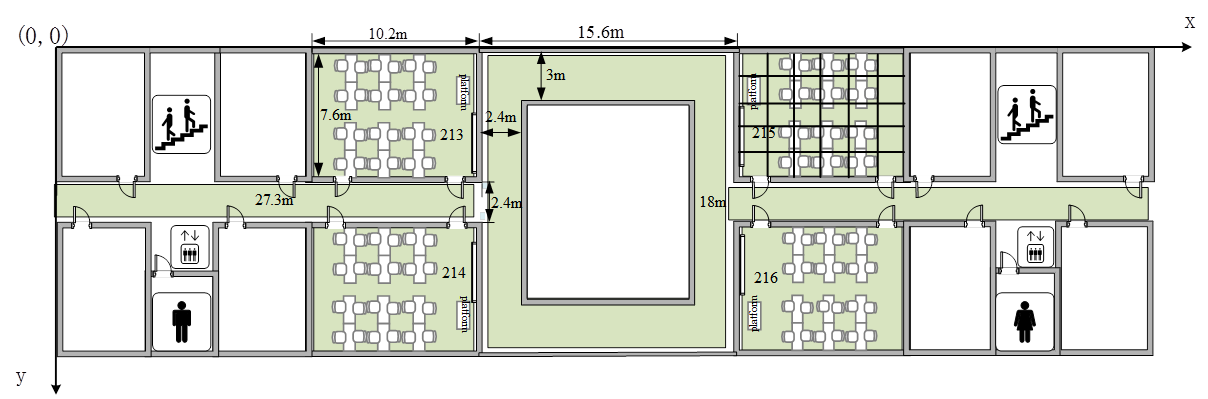
\includegraphics[width=12cm]{nanyi.png}
        \caption{南一楼局部区域室内布局图}\label{nanyi}
      \end{figure}
  \item 训练集一共有14798个样本,为了模拟实际场景中收集的样本标注位置存在误差,因此给每个样本的实际坐标添加一定的扰动。具体地,x,y轴分别添加的扰动为:均值为0,标准差为1.2m的一组随机生成的值。训练集中共接收到577个BSSID,文件中‘负值’表示相应样本接收到相应BSSID的信号强度值,'0值'表示相应样本未接收到该BSSID的值。文件中$x,y$分别表示样本实际采集位置添加扰动后的坐标。
  \item 测试集一共包括652个测试指纹,每个测试指纹是10个测试样本的均值,测试集共接收到458个BSSID。
\end{itemize}

\section{问题分析}
\begin{itemize}
  \item 首先观察训练集 $\$$ 的特征向量,发现其特征向量并不一致,故取其交集(相较与取并集预测精度有显著提高)。
  \item 对数据集中特殊点的处理:由于数据集中存在0值,可将其变为极弱信号(-100)以便于算法预测精度的提升。
  \item 算法选择方面:考虑该具体问题的性质,虽然是回归问题,但不适合使用svm、neural network等强拟合算法。外加噪声会极大地影响其效果,平均可在一定程度上弱化噪声的影响,但综合考虑使用K个最近邻样本输出的平均值作为回归预测值(KNN)即简单高效,避免复杂计算,又可以得到不错的结果,为上策。
\end{itemize}

\section{算法设计}
\begin{itemize}
  \item main-idea: 用K个最近邻样本输出的平均值作为回归预测值。
\end{itemize}

\section{Python Code for Location Assignment}
\subsection{data}
\begin{lstlisting}[language=python]
# -*- coding: utf-8 -*-
"""
@author : Haoran You

"""
import csv
import random
import numpy as np

def getFeat():
    # train datasest
    trainDT = csv.reader(open('train.csv', 'r'))
    dataset = []
    for line in trainDT:
        dataset.append(line)
    train_feat_index = dataset[0][1:-2]
    del (dataset[0])
    # test dataset
    testDT = csv.reader(open('test.csv', 'r'))
    test_feature = []
    for line in testDT:
        test_feature.append(line)
    test_feat_index = test_feature[0][1:]
    del (test_feature[0])
    # all feature
    all_feat = list(set(train_feat_index).intersection(set(test_feat_index)))
    train_index, test_index = [], []
    for item in train_feat_index:
        if item in all_feat:
            train_index.append(all_feat.index(item))
        else:
            train_index.append(-1)
    for item in test_feat_index:
        if item in all_feat:
            test_index.append(all_feat.index(item))
        else:
            test_index.append(-1)
    num_feat = len(all_feat)
    return num_feat, train_index, test_index, dataset, test_feature

def traincsv(dataset, train_index, num_feat):
    feature = []; x = []; y = []
    for item in dataset:
        feature.append(item[1:-2])
        x.append(item[-2])
        y.append(item[-1])
    feature = [[float(j) for j in i] for i in feature]
    train_feature = []
    for i in range(len(feature)):
        _feature = list(np.zeros(num_feat))
        for j in range(len(feature[i])):
            if feature[i][j] < 0.0:
                if train_index[j] == -1:
                    pass
                else:
                    # _feature[train_index[j]] = 1.0
                    _feature[train_index[j]] = feature[i][j]
            else:
                if train_index[j] == -1:
                    pass
                else:
                    _feature[train_index[j]] = -100
        train_feature.append(_feature)
    x = [float(i) for i in x]
    y = [float(i) for i in y]
    return train_feature, x, y

def testcsv(feature, test_index, num_feat):
    for i in range(len(feature)):
        feature[i] = feature[i][1:]
    feature = [[float(j) for j in i] for i in feature]
    test_feature = []
    for i in range(len(feature)):
        _feature = list(np.zeros(num_feat))
        for j in range(len(feature[i])):
            if feature[i][j] < 0.0:
                if test_index[j] == -1:
                    pass
                else:
                    # _feature[test_index[j]] = 1.0
                    _feature[test_index[j]] = feature[i][j]
            else:
                if test_index[j] == -1:
                    pass
                else:
                    _feature[test_index[j]] = -100
        test_feature.append(_feature)
    return test_feature

def divideTrainVal(feature, x, y, ratio):
    num_dataset = len(x)
    index_train = random.sample(range(num_dataset), int(num_dataset*ratio))
    train_feature, train_x, train_y = [], [], []
    val_feature, val_x, val_y = [], [], []
    for i in range(num_dataset):
        if i in index_train:
            train_feature.append(feature[i])
            train_x.append(x[i])
            train_y.append(y[i])
        else:
            val_feature.append(feature[i])
            val_x.append(x[i])
            val_y.append(y[i])
    return train_feature, train_x, train_y, val_feature, val_x, val_y

def dataset():
    num_feat, train_index, test_index, dataset, test_feature = getFeat()
    feature, x, y = traincsv(dataset, train_index, num_feat)
    train_feature, train_x, train_y, val_feature, val_x, val_y = \
    divideTrainVal(feature[:], x[:], y[:], ratio=0.9)
    test_feature = testcsv(test_feature, test_index, num_feat)
    print('num of trainset : ', len(train_feature))
    print('num of valset   : ', len(val_feature))
    print('num of testset  : ', len(test_feature))
    print('total features  : ', num_feat)
    return train_feature, train_x, train_y, val_feature, val_x, val_y, test_feature

\end{lstlisting}

\subsection{Main}
\begin{lstlisting}[language=python]
# -*- coding: utf-8 -*-
"""
@author : Haoran You

"""
import os
import csv
from data import *
import matplotlib.pyplot as plt

# load data
train_feat, train_x, train_y, val_feat, val_x, val_y, test_feat = dataset()

# train
def calDistance(x, y):
    return np.sqrt(np.square(x) + np.square(y))
def method(model_x, model_y):
    model_x.fit(train_feat, train_x)
    score = model_x.score(val_feat, val_x)
    result_val_x = model_x.predict(val_feat)
    result_test_x = model_x.predict(test_feat)
    print('score of val_x : ', score)
    model_y.fit(train_feat, train_y)
    score = model_y.score(val_feat, val_y)
    result_val_y = model_y.predict(val_feat)
    result_test_y = model_y.predict(test_feat)
    print('score of val_y : ', score)
    print('average deviation of val_x : ', np.average(abs(val_x - result_val_x)))
    print('average deviation of val_y : ', np.average(abs(val_y - result_val_y)))
    print('average deviation of val distance : ', np.average(calDistance(val_x - result_val_x, val_y - result_val_y)))
    if os.path.exists('result.csv'):
        os.remove('result.csv')
    f = open('result.csv', 'a', newline='')
    csv_write = csv.writer(f, dialect='excel')
    for i in range(len(result_test_x)):
        result = []
        result.append(i)
        result.append(result_test_x[i])
        result.append(result_test_y[i])
        csv_write.writerow(result)

    # plot val result figure
    plt.figure(1)
    plt.subplot(131)
    plt.plot(train_x, train_y, 'ro', label='real')
    plt.title('trainset distribution')
    plt.xlabel('x'); plt.ylabel('y')
    plt.legend(loc='upper right', ncol=1)
    plt.subplot(132)
    plt.plot(val_x, val_y, 'ro', label='real')
    plt.plot(result_val_x, result_val_y, 'bo', label='predict')
    plt.title('valset distribution')
    plt.xlabel('x'); plt.ylabel('y')
    plt.legend(loc='upper right', ncol=1)
    plt.subplot(133)
    plt.plot(result_test_x, result_test_y, 'bo', label='predict')
    plt.title('testset distribution')
    plt.xlabel('x'); plt.ylabel('y')
    plt.legend(loc='upper right', ncol=1)
    plt.show()

def run(type):
    if type == 'decision_tree':
        from sklearn import tree
        model = tree.DecisionTreeRegressor()
    elif type == 'linear':
        from sklearn import linear_model
        model = linear_model.LinearRegression()
    elif type == 'svm':
        from sklearn import svm
        model = svm.SVR()
    elif type == 'KNN':
        from sklearn import neighbors
        model = neighbors.KNeighborsRegressor()
    elif type == 'random_forest':
        from sklearn import ensemble
        model = ensemble.RandomForestRegressor(n_estimators=20)
    elif type == 'adaboost':
        from sklearn import ensemble
        model = ensemble.AdaBoostRegressor(n_estimators=50)
    elif type == 'extra_tree':
        from sklearn.tree import ExtraTreeRegressor
        model = ExtraTreeRegressor()
    method(model, model)

run('KNN')
\end{lstlisting}

\section{结果讨论}
\subsection{Location Distribution}
\begin{figure}[!htbp]
  \centering
  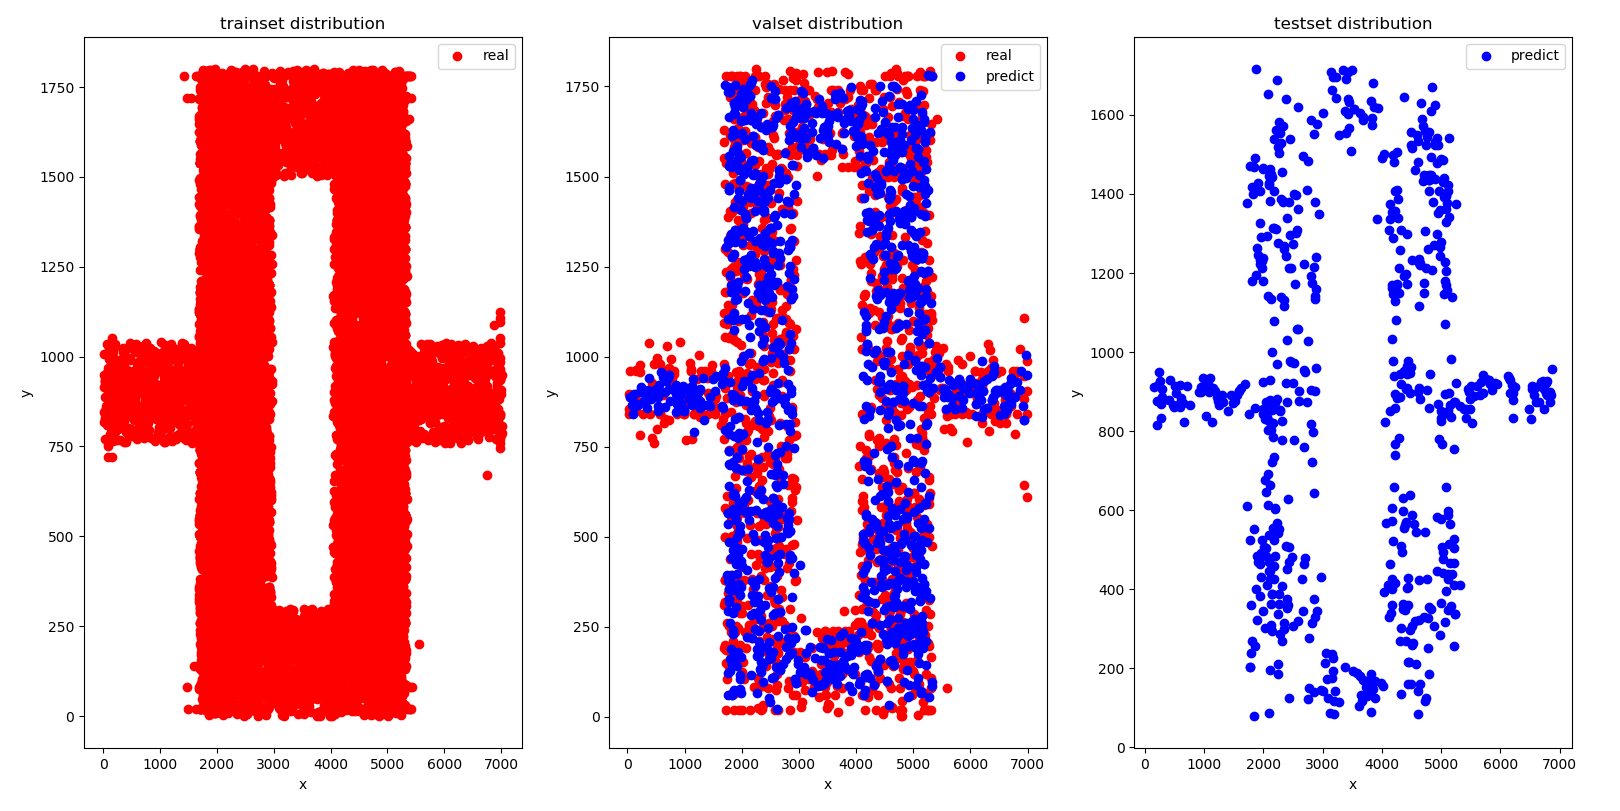
\includegraphics[width=15cm]{distribution.png}
  \caption{Location Distribution}
\end{figure}

\subsection{CDF}
\emph{CDF}为累计分布函数,结果的平均定位误差为:
\begin{equation}\label{ep:eqs}
  err = \frac{\sum_{n=1}^{N} \sqrt{(x_n^e - x_n)^2 + (y_n^e - y_n)^2}}{N}
\end{equation}
结果如图\ref{CDF}所示。

\begin{figure}
  \centering
  \begin{minipage}[t]{7.5cm}
    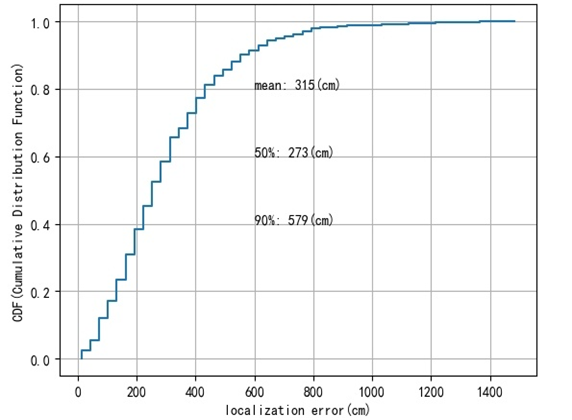
\includegraphics[width=7cm]{cdf_union.png}
    \centerline{Union feature set}
  \end{minipage}
  \begin{minipage}[t]{7.5cm}
    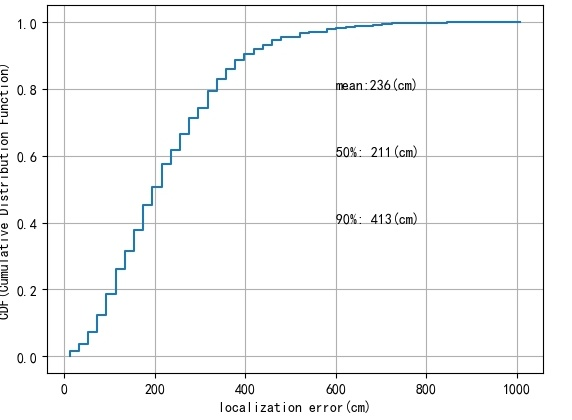
\includegraphics[width=7cm]{cdf.png}
    \centerline{Intersection feature set}
  \end{minipage}
  \caption{Cumulative Distribution Function}
  \label{CDF}
\end{figure}

\section{课程评价}
\begin{itemize}
  \item 老师准备得很细,看得出画了很大的功夫,但是讲课风格不合我的口味,我比较偏向于原理部分而不是繁琐的计算,老师在讲原理的时候没有讲得很深入或者很形象,可以考虑将课堂的计算换成更简单但也能体现原理的算例。
  \item 课后作业还可以,编程作业做了还是有收获的。但是Neural Network作业貌似没布置。
  \item 作为学院的第一次尝试来讲可以了。
\end{itemize}

\end{document} 